%%%%%%%%%%%%%%%%%%%%%%%%%%%%%%%%%%%%%%%%%
% Journal Article
% LaTeX Template
% Version 2.0 (February 7, 2023)
%
% This template originates from:
% https://www.LaTeXTemplates.com
%
% Author:
% Vel (vel@latextemplates.com)
%
% License:
% CC BY-NC-SA 4.0 (https://creativecommons.org/licenses/by-nc-sa/4.0/)
%
% NOTE: The bibliography needs to be compiled using the biber engine.
%
%%%%%%%%%%%%%%%%%%%%%%%%%%%%%%%%%%%%%%%%%

%----------------------------------------------------------------------------------------
%	PACKAGES AND OTHER DOCUMENT CONFIGURATIONS
%----------------------------------------------------------------------------------------


\documentclass[
	a4paper, % Paper size, use either a4paper or letterpaper
	10pt, % Default font size, can also use 11pt or 12pt, although this is not recommended
	unnumberedsections, % Comment to enable section numbering
	twoside, % Two side traditional mode where headers and footers change between odd and even pages, comment this option to make them fixed
]{LTJournalArticle}


\usepackage{graphicx}
\usepackage{subcaption}
\usepackage{float}
\usepackage{makecell}
\usepackage{adjustbox}
\usepackage{caption}
\usepackage{amsmath}
\usepackage{stmaryrd}


\addbibresource{sample.bib} % BibLaTeX bibliography file

\runninghead{Shortened Running Article Title} % A shortened article title to appear in the running head, leave this command empty for no running head

\footertext{\textit{Journal of Biological Sampling} (2024) 12:533-684} % Text to appear in the footer, leave this command empty for no footer text

\setcounter{page}{1} % The page number of the first page, set this to a higher number if the article is to be part of an issue or larger work

%----------------------------------------------------------------------------------------
%	TITLE SECTION
%----------------------------------------------------------------------------------------

\title{An Article Title That Spans Multiple\\ Lines to Show Line Wrapping} % Article title, use manual lines breaks (\\) to beautify the layout

% Authors are listed in a comma-separated list with superscript numbers indicating affiliations
% \thanks{} is used for any text that should be placed in a footnote on the first page, such as the corresponding author's email, journal acceptance dates, a copyright/license notice, keywords, etc
\author{%
	John Smith\textsuperscript{1,2}, Robert Smith\textsuperscript{3} and Jane Smith\textsuperscript{1}\thanks{Corresponding author: \href{mailto:jane@smith.com}{jane@smith.com}\\ \textbf{Received:} October 20, 2023, \textbf{Published:} December 14, 2023}
}

% Affiliations are output in the \date{} command
\date{\footnotesize\textsuperscript{\textbf{1}}School of Chemistry, The University of Michigan\\ \textsuperscript{\textbf{2}}Physics Department, The University of Wisconsin\\ \textsuperscript{\textbf{3}}Biological Sciences Department, The University of Minnesota}

% Full-width abstract
\renewcommand{\maketitlehookd}{%
	\begin{abstract}
		\noindent Lorem ipsum dolor sit amet, consectetur adipiscing elit. Praesent porttitor arcu luctus, imperdiet urna iaculis, mattis eros. Pellentesque iaculis odio vel nisl ullamcorper, nec faucibus ipsum molestie. Sed dictum nisl non aliquet porttitor. Etiam vulputate arcu dignissim, finibus sem et, viverra nisl. Aenean luctus congue massa, ut laoreet metus ornare in. Nunc fermentum nisi imperdiet lectus tincidunt vestibulum at ac elit. Nulla mattis nisl eu malesuada suscipit. Aliquam arcu turpis, ultrices sed luctus ac, vehicula id metus. Morbi eu feugiat velit, et tempus augue. Proin ac mattis tortor. Donec tincidunt, ante rhoncus luctus semper, arcu lorem lobortis justo, nec convallis ante quam quis lectus. Aenean tincidunt sodales massa, et hendrerit tellus mattis ac. Sed non pretium nibh. Donec cursus maximus luctus. Vivamus lobortis eros et massa porta porttitor.
	\end{abstract}
}

%----------------------------------------------------------------------------------------

\begin{document}

\maketitle % Output the title section

%----------------------------------------------------------------------------------------
%	ARTICLE CONTENTS
%----------------------------------------------------------------------------------------

\section{Introduction}

\subsection{Contexte}

Les algorithmes de \textit{computer vision} pour la détection de points d'intérêt sont aujourd'hui extrêmement efficaces, en particulier depuis la publication de SIFT [\ref{cite:sift}] en 2004, avec des applications dans de nombreux domaines : médecine, logistique et imagerie numérique pour ne citer qu'eux.
Néanmoins, les algorithmes existants semblent inadaptés lorsqu'il s'agit de traiter des images sous-marines, et ce principalement à cause de la perte de contraste et du manque de luminosité aux profondeurs considérées.
Un domaine dans lequel cette lacune est particulièrement visible est la reconstruction de coraux par images sous-marines. Des images de l'organisme marin sont prises en stéréographie à l'aide d'un robot possédant deux caméras, et une reconstitution 3D est ensuite effectuée en comparant les images prises par les deux caméras pour déterminer la profondeur de chaque point dans les images.
Cette détermination de la profondeur passe par un \textit{matching} entre les deux images : pour certains points notables dans l'image de gauche, appelés points d'intérêt, le point correspondant sur l'image de droite doit être trouvé.
Pour avoir une grande précision dans cette reconstitution ($< 1$mm, ce qui n'est pas atteint à l'heure actuelle), il est nécessaire d'avoir un grand nombre de points ($N \approx 3000$ sur des images de résolution $3000 \times 2000$) dont la correspondance est exacte.
Or SIFT donne un très grand nombre de correspondances ($N \approx 3000$) sur ce type d'images, mais dont un très grand nombre sont erronées, ce qui fait baisser la précision de la reconstruction d'un facteur $10$, voire plus.
Nous avons donc souhaité améliorer la détection et la caractérisation de points d'intérêt dans des images sous-marines pour pouvoir augmenter la précision des méthodes de reconstitution d'organismes sous-marins, qui sont amenées à se développer aujourd'hui pour faire face à la perte massive de récifs coraliens.

\subsection{Objectif}

Notre objectif a été d'améliorer le taux de détection de "bons" points d'intérêt par rapport à l'algorithme SIFT. Des "bons" points sont des points qui correspondent de manière non équivoque et au pixel près au même point dans le monde réel.
Pour cela, nous avons été amenés à définir ce qui caractérisait un point d'intérêt, et à définir des métriques objectives et quantitatives permettant de comparer les algorithmes sur la détection et la correspondance de points d'intérêt.

%------------------------------------------------
\section{Etat de l'art}

Dans cette section, nous présentons les algorithmes de détection et caractérisation de points d'intérêt déjà développés dans la littérature.

Parler des cross-correlation, du fait que ce n'était pas assez puissant.

\subsection{SIFT}

SIFT (\textit{Scale Invariant Feature Transform}) [\ref{article:sift}], algorithme fondateur dans le domaine, utilise les extrema de l'espace des échelles pour déterminer des points d'intérêt dans l'image.
L'espace des échelles de l'image est calculé en effectuant des différences de gausiennes, i.e. des différences pixel par pixel de l'image convoluée par des filtres gaussiens d'écart-type $\sigma$ variable.
Un pixel à une échelle $\sigma_i$ est alors considéré comme un point d'intérêt si et seulement si sa valeur est supérieure (resp. inférieure) aux 8 pixels voisins à l'échelle $\sigma_i$, aux 9 pixels voisins à l'échelle $\sigma_{i+1}$ et aux 9 pixels voisins à l'échelle $\sigma_{i-1}$ (c'est alors un extremum de l'espace des échelles).
Après une étape de filtrage intermédiaire, les points d'intérêt trouvés sont alors caractérisés par un histogramme d'orientation des gradients autour du point.
Le détail de l'assignation d'une orientation et d'une magnitude aux gradients des voisins est donné par les équations %\ref{eq:gradient_orientation}.
Chaque point d'intérêt est ainsi représenté par un descripteur de dimension 128, contenant les informations d'un carré de 4x4 histogrammes autour du point, avec 8 directions enregistrées dans chaque cellule. (INSERER IMAGE p.15 article SIFT)

% \begin{figure}
% 	\centering
% 	\begin{subfigure}[H]{\columnwidth}
% 		\centering
% 		\includegraphics[width=\textwidth]{images/sift_descriptor.png}
% 	\end{subfigure}
% 	\label{figure:sift_descriptor}
% 	\caption{Illustration du descripteur utilisé dans SIFT}
% \end{figure}

\subsection{SURF}

\subsection{DAISY}

Rapide + wide baseline

\section{Données}

Dans cette section, nous présentons les images que nous avons à traiter dans le cadre de la stéréographie sous-marine.

\subsection{Images réelles}

Les images réelles dont nous disposons proviennent d'une expérience en bassin peu profond, dans lequel un rocher de dimensions approximatives 30 cm $\times$ 20 cm $\times$ 20 cm a été photographié par un robot à deux caméras. Un exemple d'image est disponible en figure \ref{figure:irl_example}.
Les différences majeures entre des images en surface et des images sous-marines sont une perte de contraste significative et une modification des couleurs (visible à l'oeil nu).

% \begin{figure}
% 	\centering
% 	\begin{subfigure}[H]{\columnwidth}
% 		\centering
% 		\includegraphics[width=\textwidth]{images/irl_example.png}
% 	\end{subfigure}
% 	\label{figure:irl_example}
% 	\caption{Une image réelle expérimentale}
% \end{figure}

Les paramètres des images et des caméras sont donnés ici.
Les images sont de résolution XX, l'angle entre les caméras nous a été estimé à 10°, les caméras sont situés à environ 1m du rocher, et elles ont une distance focale de XX mm.

\subsection{Images de synthèse}

DONNER DIMENSIONS ROCHER

Pour pouvoir comparer les performances des descripteurs de l'état de l'art et le descripteur que nous avons conçu, nous avons décidé de créer des images de synthèse à l'aide du logiciel open-source Blender [\ref{cite:blender}], pour créer une scène 3D dans laquelle tous les paramètres seraient connus.
Un rocher texturé a été simulé dans cette scène 3D à l'aide de déformations à bruit gaussien, et deux caméras ont été placées pour simuler la stéréographie sous-marine.
Les scènes sont disponibles sur le dépôt du projet, nous donnons ici les principaux paramètres des scènes en table \ref{table:params_syn_imgs}

\begin{table*}[t]
	\begin{adjustbox}{width=\columnwidth, left}
		\begin{tabular}{l c}
			\hline
			Résolution          & ??    \\
			\hline
			Angle entre caméras & $10$° \\
			Distance focale     & ??    \\
			Distance à l'objet  & 1m    \\
			\hline
		\end{tabular}
	\end{adjustbox}
	\label{table:params_syn_imgs}
	\caption{Paramètres des images de synthèse (A MODIFIER)}
\end{table*}

Ces images de synthèse permettent de comparer des points d'intérêt trouvés de manière informatique, en vérifiant si les correspondances sont bonnes grâce à Blender.
Pour ce faire, pour chaque caméra, nous traçons les rayons partant du centre de la caméra, passant par le point trouvé, et nous enregistrons le point de collision entre ce rayon et le rocher simulé.
La distance (3D) entre ces points de collision donne une métrique continue de la qualité du \textit{match}, qui peut être ensuite transormée en une métrique binaire (bon/mauvais \textit{match}) en mettant un seuil de distance, qui peut être variable, et qui correspond à la distance entre deux pixels au point considéré.


(Rajouter pas de filtrage droite épipolaire car long à implémenter par rappport à Blender + long à faire tourner sur grosses images)

(RAJOUTER IMAGE VERIFICATION BLENDER)

\section{Méthodologie}

\subsection{Traitement de l'image}
Les images sont transformées en niveau de gris par simple moyenne des $3$ canaux de couleur \textit{RGB}.
Un recadrage manuel est effectué pour enlever au maximum les pixels de l'arrière-plan, car les points
d'intérêts sont à chercher sur l'objet photographié. Ensuite un filtre gaussien est
appliqué, d'écart-type $1$ et uniquement sur les images de synthèse, car les images réelles
ont peu de contraste. En réponse, des méthodes d'augmentation
de contraste ont été testées, aucune amélioration notable n'a été constatée.


\subsection{Notion de point d'intérêt}

Il est certes possible de chercher les paires de points de façon brute entre
l'entièreté des pixels de chaque image, mais c'est insensé sur le
point de vue du temps de calcul, et clairement inutile: beaucoup de
points réels ne présentent que peu d'intérêt car leur voisinage présente
peu de relief.

La question est alors de définir un bon point
d'intérêt, ie un point dont le voisinage topologique varie de façon
assez significative pour être reconnaissable sur les deux images.
Un changement de point d'observation s'effectue pendant
la prise de celles-ci, changeant alors le relief apparent et le contraste.

Pour la caractérisation des points, SIFT se concentre sur la répartition des gradients
dans le voisinage. Il élimine avant cela les points sur des arêtes, jugés trop
sensibles au bruit, il calcule pour cela la trace et le déterminant
de la hessienne, fonctions des courbures principales.

Les courbures principales sont les extrema des courbures en un point.
Elles coïncident avec les valeurs propres de la hessienne de la surface en le point,
et leurs directions respectives sont les vecteurs propres associés.

Ces courbures principales et leur directions mériteraient plus d'attention,
et pourraient être considérées telles quelles. Dit grossièrement,
elles contiennent une information à l'ordre $2$ sur la surface et complètent
l'information d'ordre $1$ fournie par le gradient. Un bon
point d'intérêt a selon nous dans son voisinage une variation marquée des courbures.


C'est pour cela qu'un préfiltrage grossier est fait: sur chaque image,
seul $30 \%$ des pixels de plus grande courbure principale moyenne (en norme)
sont gardés.

\subsection{Descripteur}
Comme dans SIFT un descripteur est construit,
son but est d'encoder dans un vecteur des caractéristiques topologiques de son voisinage, qu'on espère trouver
sur les deux images le plus à l'identique possible.

Définissons d'abord des propriétés de robustesse
que nous souhaitons pour notre descripteur:

\begin{enumerate}
	\item Invariance par rotation: le robot sous-marin n'est pas parfaitement
	      horizontal lorsqu'il photographie. Une même forme n'aura pas la même
	      orientation sur les deux images. Nous souhaitons donc pouvoir identifier un
	      point, même si son voisinage subit une rotation dans le plan de photographie.
	\item Robustesse à la luminosité: la lumière sous-marine est naturellement inégale,
	      que ce soit à cause de la lumière du soleil qui est réfractée dans l'eau
	      et réfléchie sur les particules sous-marines, ou bien à
	      cause des éclairages du robot sous-marin.
\end{enumerate}

Il est important de souligner que l'invariance par échelle, propriété essentielle de SIFT,
n'a pas été implémentée. La raison est que cette propriété
répond à un besoin très général d'identifier des points d'intérêt à différentes
échelles. C'est très utile lorsque l'objet ciblé présente une structure et
un relief très variés, par exemple une maison. Mais dans notre utilisation précise,
nous voulons à terme photographier des récifs coraliens, et actuellement, en
phase expérimentale, nous utilisons des rochers. Le relief d'un rocher ne présente
pas de motif notable, comme des arêtes marquées, mais tend au contraire à être
uniforme et répétitif.

Il semble raisonnable de tirer parti de la
constance du dispositif expérimental, pour trouver assez de bons points ($N > 3000$)
en comparant des voisinages d'une même taille fixe, déterminée à l'avance.



Le descripteur repose principalement sur le gradient et les courbures principales.
Ces valeurs sont approximées par différences finies symétriques de l'image à l'ordre $1$ et $2$.
Si l'on définit une image numérique $I$ de dimension $(w, h) \in \mathbb{N}^2$,
comme une fonction discrète:
$I: \llbracket 0, w-1 \rrbracket \times \llbracket 0, h-1 \rrbracket \rightarrow [0, 1]$
d'abscisses $x$ et d'ordonnées $y$, la norme du gradient
et son orientation sont approximées par:

\begin{multline}
	m(x, y) = \\
	\sqrt{(I(x+1, y) - I(x-1,y))^2 + (I(x,y+1)-I(x,y-1))^2}
\end{multline}

\begin{multline} \label{eq:angle_grad}
	\theta(x, y) = \\
	\tan^{-1}\left(\frac{I(x,y+1)-I(x,y-1)}{I(x+1, y) - I(x-1,y)}\right)
\end{multline}

Pour calculer les courbures et directions principales, la hessienne $H$ est d'abord calculée
similairement, voir l'équation~\ref{eq:hess_coefs} en Annexes :

\begin{equation}
	H = \\
	\begin{bmatrix}
		dxx & dxy \\
		dxy & dyy
	\end{bmatrix}
\end{equation}

Puis le module \textit{Numpy} de \textit{Python} est utilisé pour en obtenir les valeurs et vecteurs
propres.
Avant de construire l'histogramme, quelques choix techniques doivent être précisés.
Dans tout l'algorithme, les angles sont dans $[0, 360]$. Afin de n'avoir que des
courbures positives, les courbures négatives sont multipliées par $-1$
et les vecteurs propres associés sont tournés de $180$°.

Le voisinage autour d'un pixel est ensuite construit. En appelant $\theta$
l'orientation du gradient en le point, le voisinage en question est l'image par
une rotation d'angle $\theta$ d'un carré de $15\times 15$ pixels, (IL MANQUE UN MOT ?)
centré en le pixel. Cela permet d'être invariant par rotation.
Ce voisinage est ensuite découpé en $9$ cellules de $25$ pixels.
D'autre tailles de voisinage n'ont pas été testées en comparaison, à
part un voisinage $5 \times 5$ qui a sans surprise donné de moins bons résultats.

Un histogramme des gradients des pixels est alors calculé en chacune des $9$ cellules .
Chaque gradient d'un voisin contribue à
l'angle correspondant à l'écart entre son orientation et celle du pixel central.
La résolution angulaire de l'histogramme est $5$°, donc celui-ci est un vecteur de taille
$360 / 5 = 72$.
La contribution d'un pixel
est le rapport entre la norme de son gradient et celle du pixel central,
seuillée à $\varepsilon = 10^{-6}$ afin d'éviter une division par $0$.
Cette contribution est pondérée par une fonction gaussienne de sa distance au centre,
d'écart type la moitié du voisinage, ici $7.5$, et ceci afin de limiter l'influence des
de la topologie aux bords du voisinage, voir la Figure~\ref{figure:lowe_desc_constr}.
Les contributions sont ensuite transformées en pourcentage
de la somme des contributions dans toutes les cellules, afin de fournir une invariance
à la luminosité. Ainsi, le tableau des $9$ histogrammes est de taille $9 \times 72 = 648$

\begin{figure}[H]
	\centering
	\begin{subfigure}[H]{\columnwidth}
		\centering
		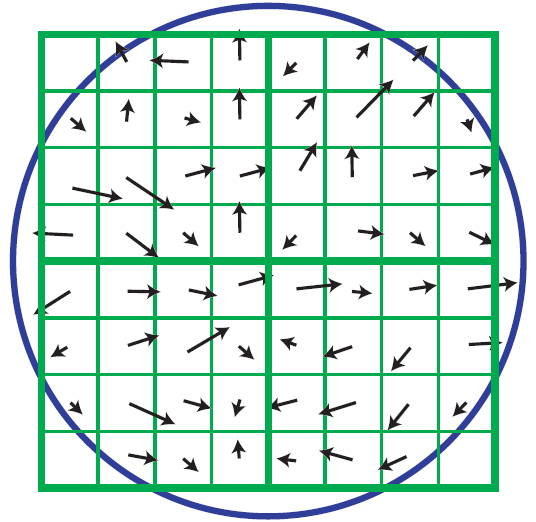
\includegraphics[width=0.6\textwidth]{images/lowe_grads.png}
	\end{subfigure}
	\begin{subfigure}[H]{\columnwidth}
		\centering
		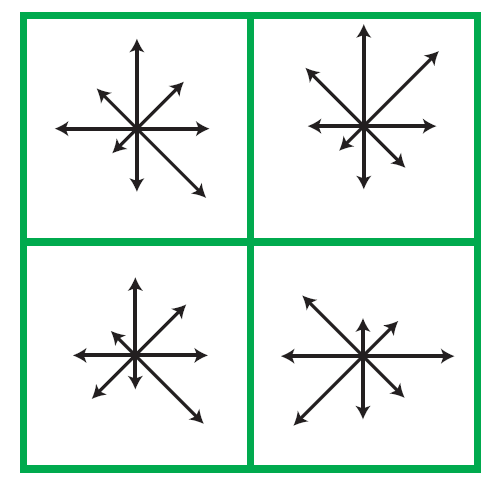
\includegraphics[width=0.55\textwidth]{images/lowe_desc.png}
	\end{subfigure}
	\caption{Schémas des gradients d'un voisinage $8 \times 8$ d'un pixel, la pondération
		gaussienne y apparaît en bleu, et des histogrammes des cellules. (Illustrations tirées
		de SIFT) }
	\label{figure:lowe_desc_constr}
\end{figure}

On calcule de la même façon les deux histogrammes des courbures principales
(ordonnées par valeur signée décroissante). Pour cela,
on définit l'orientation d'une courbure principale comme l'angle fait entre sa
direction et le vecteur horizontal $e_x=(x=1, y=0)$, et la contribution va,
comme précédemment, à l'écart entre les orientations du voisin et du pixel central.
Comme exemple, voir la Figure~\ref{figure:fig_hist} en Annexes.

En concaténant les $3$ tableaux d'histogrammes, on obtient le descripteur du pixel,
qui est un vecteur de taille $3 \times 648 = 1944$.


\subsection{Appariement}

Bien qu'il existe des méthode analogues aux plus proches voisins adaptées à de la haute dimension,
comme la \textit{Best Bin First}, elles n'ont pas utilisées car elles n'ont
pas été recréées pour le projet et celles des librairies \textit{Python} ne peuvent pas être
précompilées en \textit{C} par \textit{Numba}, module utilisé pour avoir des temps
de calcul "raisonnables".

L'appariement brut a donc été choisi: pour chaque pixel filtré de l'image de gauche,
on l'associe à celui de l'image de droite ayant le descripteur le plus similaire,
dans le sens où il minimise leur distance euclidienne.
Ce choix de distance a encore été fait par défaut et aucune autre distance
n'a été testée.

Il pourrait être intéressant d'expérimenter avec une norme pondérée, accordant plus d'importance
à l'information des gradients par rapport à celle des courbures.

\subsection{Postfiltrage}
Une fois les paires calculées, nous n'en gardons que $2 \%$ du nombre de pixels de l'image,
ayant les plus petites distances, ie les paires avec le plus haut taux
de confiance. Ce seuil a été retenu puisqu'il correspond à un peu plus que
l'objectif de $3000$ bonnes paires sur nos images réelles recadrées, de résolution
$900 \times 1400$.
Nous l'avons aussi utilisé sur nos images de synthèses, même si la résolution est inférieure.

Par commodité, on désignera notre algorithme
par \textit{HM}, pour \textit{Home Made}.

\subsection{Analyse du descripteur sur images de synthèse}

Afin de savoir si le descripteur ainsi construit permet de distinguer
des bons points d'intérêts des mauvais,
pour chaque image, la moyenne des histogrammes spatiaux de
la courbure principale $1$ des bons points parmi les paires
renvoyées par \textit{HM} est calculée. Idem pour les mauvais points, cf Figure~\ref{figure:desc_comp}.
Cependant, aucune différence notable apparaît entre le bon et mauvais descripteurs,
les différences visibles sont de l'ordre de $0.01 \%$.
Le même constat est fait pour les autres histogrammes spatiaux du
descripteur. Ces observations ne
permettent pas d'inférer un critère de sélection de bons points d'intérêt.

%------------------------------------------------

\begin{table*}[t]
	\centering
	\begin{adjustbox}{width=\textwidth,center}
		\begin{tabular}{l c c c c}
			\hline
			Angle entre caméras                                                       & \multicolumn{2}{c}{$10$°} & \multicolumn{2}{c}{$7$°}                                              \\
			Algorithme (préfiltrage)                                                  & \textit{HM} ($60\%$)      & SIFT                     & \textit{HM} ($70\%$) & SIFT                \\
			\hline\makecell[l]{Nombre de bonnes paires parmi les                                                                                                                          \\
			$3480$ de distance minimale (\% de paires)}                               & $2579$ ($74.11 \%$)       & $613$ ($17.61 \%$)       & $2532$ ($72.76 \%$)  & $604$ ($17.36 \%$)  \\
			\hline
			\makecell[l]{Statistiques sur les distances                                                                                                                                   \\
			des bonnes (B) et mauvaises (M) paires}                                   & (B)   (M)                 & (B)   (M)                & (B)   (M)            & (B)   (M)           \\
			\makecell[l]{Min}                                                         & $10.98$   $14.11$         & $27.48$   $33.18$        & $11.97$   $12.35$    & $15.56$   $38.74$   \\
			\makecell[l]{Max}                                                         & $33.69$   $44.50$         & $255.22$   $264.50$      & $32.45$   $43.46$    & $253.92$   $251.11$ \\
			\makecell[l]{Moyenne}                                                     & $20.82$   $23.24$         & $111.58$   $124.36$      & $20.79$   $23.28$    & $112.42$   $121.08$ \\
			\makecell[l]{Ecart-type}                                                  & $1.99$   $2.72$           & $49.09$   $52.81$        & $2.03$   $2.75$      & $50.70$   $48.92$   \\
			\makecell[l]{Ecart entre les distances moyennes                                                                                                                               \\
			des bonnes et mauvaises paires divisé par l'écart-type des bonnes paires} & $1.22$                    & $0.26$                   & $1.23$               & $0.17$              \\
			\hline
			\makecell[l]{Résultats avant postfiltrage (Sélection des $2\%$)}          &                           &                          &                      &                     \\
			\makecell[l]{Total de paires calculées}                                   & 69600                     & 931                      & 52200                & 930                 \\
			\makecell[l]{Total de bonnes paires renvoyées (\% de paires)}             & 17110 ($24.58\%$)         & 613 ($65.84 \%$)         & 12647($24.23\%$)     & 604   ($64.94\%$)   \\
			\hline
			\makecell[l]{Temps de calcul (hh:mm:ss) :                                                                                                                                     \\
			Image $1$, Image $2$, Appariement}                                        & \makecell{00:15:39,
			\\ 00:15:27, \\ 00:12:05}     &  Total $<5$s                       &    \makecell{00:11:48,\\ 00:11:37, \\ 00:09:24}                 &       Total $<5$s                \\
			\hline
		\end{tabular}
	\end{adjustbox}
	\caption{Comparaison des résultats sur deux paires d'images de synthèse de résolution $900 \times 1400$
		de l'algorithme \textit{HM} par rapport à SIFT réglé par défaut.
		Les bonnes paires ont été identifiée par l'algorithme Blender.}
	\label{table:res_syn}
\end{table*}


\section{Résultats}

Dans cette section, \textit{HM} est comparé avec SIFT, paramétré par défaut, ie avec un seuil de contraste de $0.04$,
un seuil d'arête de $10$, un écart type de gaussienne de $1.6$, et un seuil de distance de $0.75$.
Il aurait été intéressant d'essayer d'optimiser SIFT sur les images de synthèse
pour avoir une meilleure comparaison.
\subsection{Résultats sur image de synthèse}

Pour des sous images de synthèses de résolution $300 \times 580$ et
d'angles entre caméras de $10$° et $7$° degrés, les résultats sont dans le Tableau~\ref{table:res_syn}.
Surprenamment, \textit{HM} a d'excellents résultats: la proportion de bonnes paires parmi celles gardées
est haute par rapport à celle de SIFT.

Il est rassurant d'avoir une distance moyenne des bonnes paires en dessous de celle des mauvaises.
De plus l'écart entre les deux moyennes est d'environ $1.22$ fois l'écart-type des bonnes paires (pour $10$°). Pour SIFT en comparaison,
il est seulement de $0.27$ fois.
On en conclut que sur ce test, notre descripteur a été plus discriminant que SIFT.

Quand on regarde les résultats pour $10$° avant d'avoir fait le postfiltrage, donc avant de ne garder que l'équivalent des $2\%$ des pixels de l'image,
on voit que \textit{HM} renvoie comme attendu un grand nombre de paires, et la bonne nouvelle est que parmi elles se trouvent relativement beaucoup
de bonnes paires: $24.58\%$. A contrario, SIFT a la vertu d'être très parcimonieux et précis avec $931$ paires dont $65.8\%$ de bonnes.
Cependant, le reproche qu'on peut faire à SIFT est de ne pas renvoyer assez de bonnes paires, bien que le pourcentage de bonnes paires
parmi le nombre de pixels de la sous-image est de $0.31\%$, supérieur à l'objectif de $0.24\%$ correspondant à 3000 points dans une
image $900 \times 1400$. Ainsi, SIFT valide dans notre cas nos attentes, mais de peu, là où \textit{HM} peut potentiellemnt détecter bien
plus de bons points.

On peut voir sur la Figure~\ref{figure:fig_syn} des paires proposées par \textit{HM}.
Un effet du préfiltrage par la courbure principale moyenne est que \textit{HM} ne renvoie pas
de paires dans les zones peu contrastées, là où SIFT en trouve plus, voir Figure~\ref{figure:fig_syn_sift}
en Annexes.

\begin{figure}
	\centering
	\begin{subfigure}[H]{\columnwidth}
		\centering
		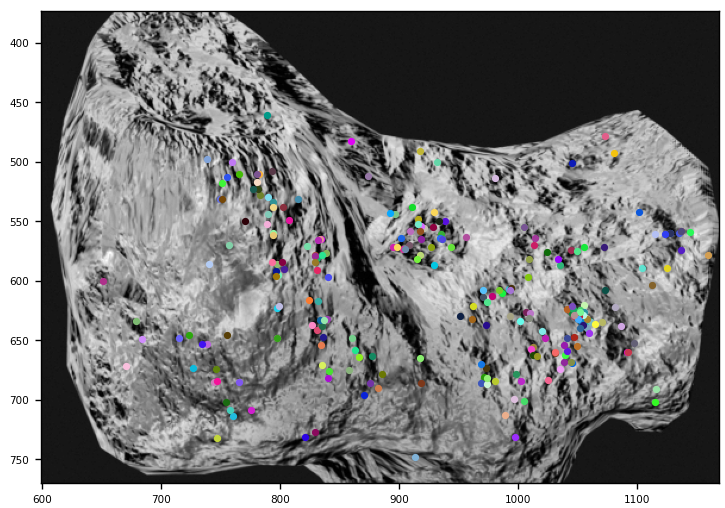
\includegraphics[width=\textwidth]{images/res1_g.png}
	\end{subfigure}

	\begin{subfigure}[H]{\columnwidth}
		\centering
		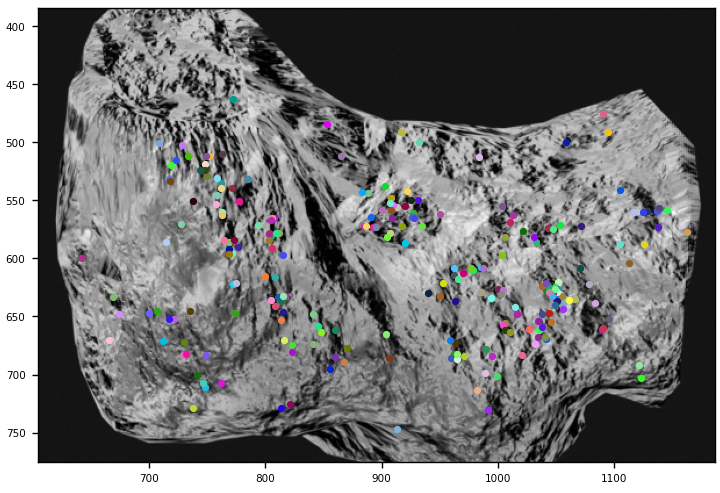
\includegraphics[width=\textwidth]{images/res1_d.png}
	\end{subfigure}
	\caption{$250$ paires tirées aléatoirement parmi celles proposées par \textit{HM}.}
	\label{figure:fig_syn}
\end{figure}

\begin{figure*}
	\centering
	\begin{subfigure}[H]{0.45\textwidth}
		\centering
		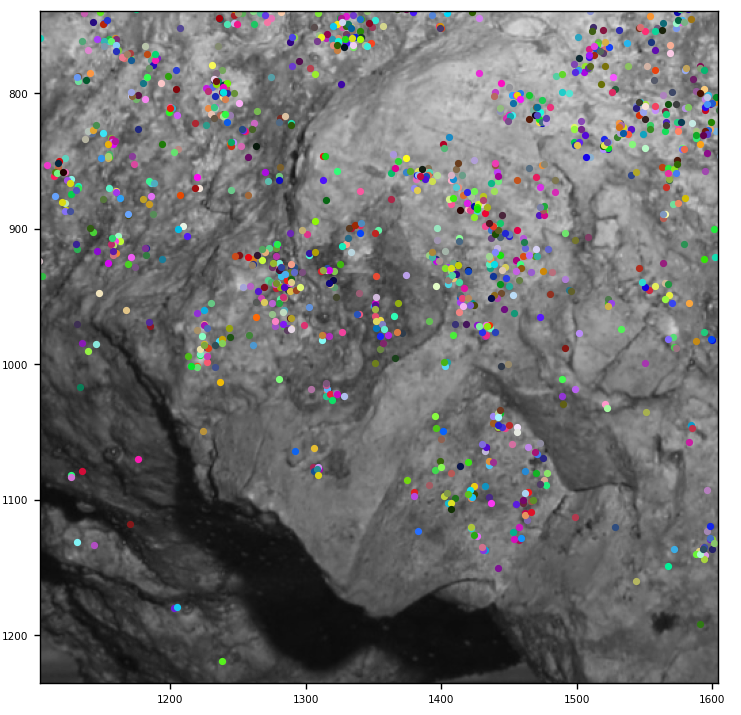
\includegraphics[width=\textwidth]{images/irl_z2_g.png}
	\end{subfigure}
	\hfill
	\begin{subfigure}[H]{0.45\textwidth}
		\centering
		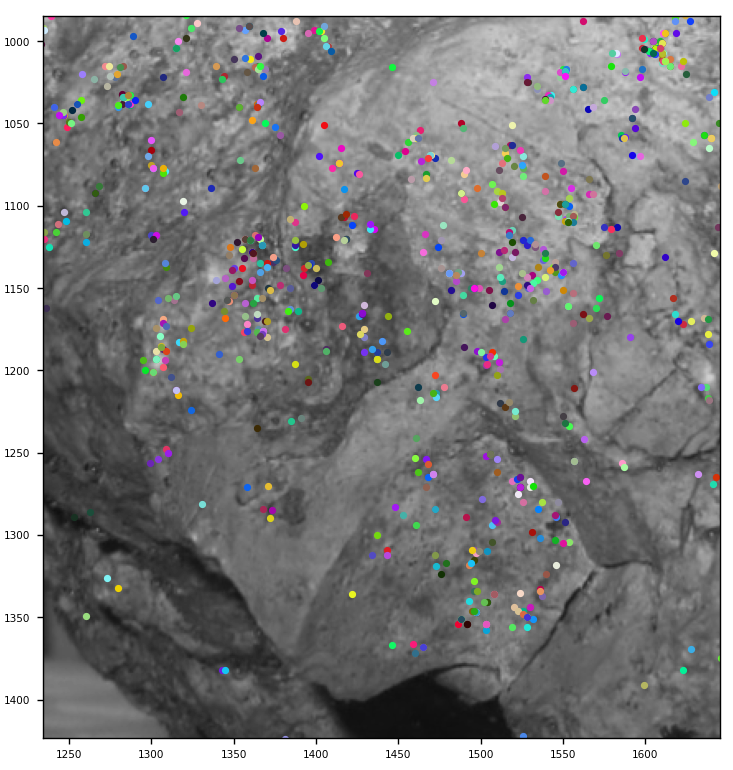
\includegraphics[width=\textwidth]{images/irl_z2_d.png}
	\end{subfigure}
	\caption{Zoom sur des paires tirées aléatoirement parmi celles proposées par \textit{HM} sur images réelles.}
	\label{figure:fig_irl}
\end{figure*}

\subsection{Résultats sur images réelles}
Les images réelles dont nous disposons ont comme résolution $800 \times 1500$ après recadrage. \textit{HM} a fonctionné
avec un préfiltrage de $70 \%$, le temps de calcul a été de 4 heures 30 par image et 5 heures 10 pour l'appariement.
On voit clairement ici la limite de notre algorithme, peu parcimonieux par nature et implémenté en Python.
Quant aux résultats, les zooms en Figure~\ref{figure:fig_irl} montrent de nombreux déchets, malgré de visiblement
bonnes paires dans les zones contrastées.
On voit tout d'abord que les images de synthèses sont sensiblement différentes des réelles,
en terme d'angle entre caméras, de variation de contraste, et de résolution.
On comprend ici la faiblesse de \textit{HM} sur ces dernières qui semble observer un voisinage fixe,
trop petit ici pour encapsuler un relief topologique caractéristique du point,
car ces images sont de haute résolution et possèdent globalement peu de relief, donc les
variations notables de celui-ci se font sur une plus grande zone que $15 \times 15$.
On trouvera en Annexes sur la Figure~\ref{figure:fig_irl_sift} les résultats de SIFT sur la même zone.
Sans surprise, ceux-ci sont très bons, avec très peu de déchets flagrants, il faudrait certes zoomer plus
pour vérifier la validité des paires au pixel près, mais il reste que les performances de \textit{HM}
restent bien en deçà de celles de SIFT. S'il faut néanmoins trouver un avantage à \textit{HM}, on fera
remarquer que celui-ci a trouvé quelques visiblement bonnes paires, non identifiées par SIFT, par
exemple la paire bleue en bas à gauche de la Figure~\ref{figure:fig_irl}.
Mais évidemment, l'algorithme \textit{HM} n'a pas les résultats attendus.


% \clearpage

\section{Discussion}

Une lacune importante de notre méthodologie est que les différents paramètres
n'ont pas été testés avec d'autres valeurs pour s'assurer que celles
utilisées sont les plus pertinentes.
C'est par exemple le cas pour l'écart-type du filtre gaussien
lors du traitement d'image, influant sur l'équilibre détail - bruit;
la résolution, les dimensions des rochers, l'éclairage et l'angle de caméras des images de synthèse,
pas assez proches de ceux des images réelles;
le pourcentile de points à garder pour l'appariement;
ou plus important encore, la taille du voisinage pour le descripteur.\\

Ce dernier point semble important car l'algorithme \textit{HM} repose sur l'hypothèse
de pouvoir trouver assez de bons points avec une taille fixe de voisinages. Or celle-ci
n'a pas fait l'objet d'un travail spécifique de détermination, et la valeur retenue de $15$
est arbitraire et trop petite pour la résolution des images réelles.

Une méthode pour pallier cela serait d'abord d'ajuster, comme évoqué juste avant, les paramètres des
images de synthèse, afin d'avoir des scènes virtuelles plus fidèles à la réalité, ensuite
observer la variation du taux de bonnes paires trouvées par \textit{HM} en fonction de la taille du descripteur. C'est au final une tâche d'optimisation.
Il est fort probable que cette relation soit une fonction croissante,
il faudrait sûrement introduire une pénalité ou une limite
supérieure sur la taille.
En plus de cela, l'étape de préfiltrage est grossière: il serait pertinent d'inclure
la norme du gradient en plus des courbures. Cette remarque vaut aussi pour l'étape
d'appariement par distance entre descripteurs, distance pouvant être
pondérée pour augmenter l'importance de l'information sur les gradients par rapport
à celle des courbures.
Il serait aussi envisageable, une fois la taille de descripteur fixée, de s'inspirer
encore de SIFT et d'ajouter une étape de détection d'extrema
locaux sur des différences de gaussiennes. A la différence qu'on se limiterait à
un nombre restreint d'échelles, choisies en fonction de la taille du descripteur.
On pourrait même incorporer la phase d'interpolation des extrema dans l'espoir
d'ajouter de la précision.

Enfin, comme présenté en introduction, plusieurs méthodes très efficaces ont été développées
ces dernières années à la suite de \textit{SIFT}, comme \textit{SURF} et \textit{DAISY}.
Elles n'ont pas été utilisées pour ce travail mais semblent pertinentes.

\section{Remerciements}

Nous tenons à remercier tous les encadrants du trimestre \textit{Data Sophia}
pour leur aide et leurs conseils: Philippe Blanc pour ses cours sur le traitement d'image,
Sébastien Travadel pour ses cours sur l'apprentissage statistique et son encadrement de notre travail,
Luca Istrate pour son aide informatique, Frank Guarnieri et Hadrien Verbois pour son cours sur
les séries temporelles.

\clearpage

\section{Annexes}

\begin{equation} \label{eq:hess_coefs}
	\begin{split}
		dxx & = I(x+1, y) + I(y, x-1) - 2I(x, y),                                              \\
		dyy & = I(x, y+1) + I(y-1, x) - 2I(x, y),                                              \\
		dxy & = \frac{\left(I(x+1; y+1) + I(x-1, y-1) - I(x-1, y+1) - I(x+1, y-1) \right)}{4}.
	\end{split}
\end{equation}

\begin{figure}[H]
	\centering
	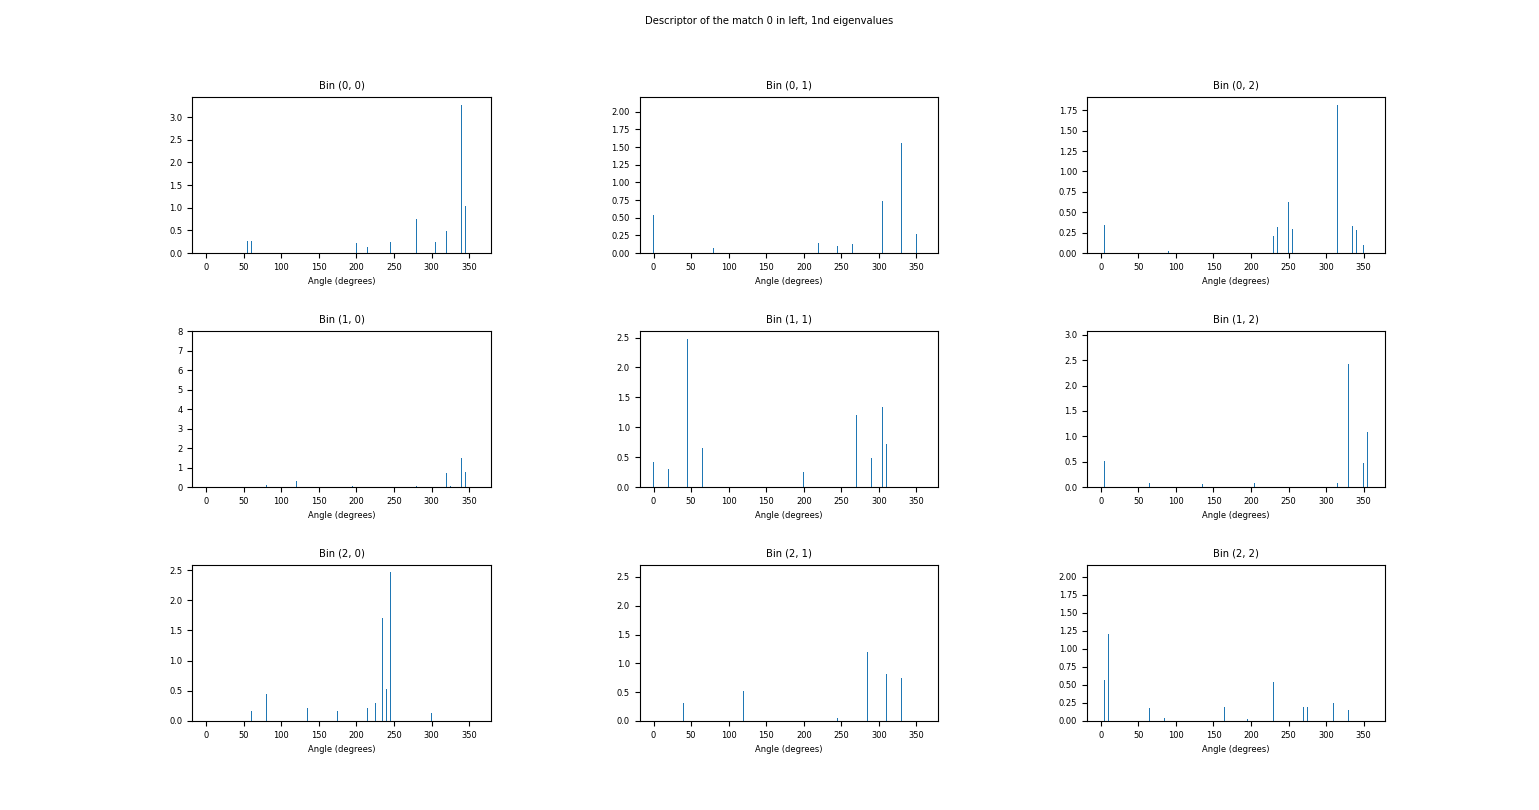
\includegraphics[width=\textwidth]{images/histo_result.png}
	\caption{Exemple du tableau des histogrammes de la courbure principale $2$,
		servant à construire le descripteur d'un point. Les bins désignent les différentes
		cellules, la $(0,0)$ est en haut à gauche de la $(1,1)$, contenant en son
		centre le point pour lequel le descripteur est calculé.}
	\label{figure:fig_hist}
\end{figure}

\begin{figure*}
	\centering
	\begin{minipage}{\textwidth}
		\centering
		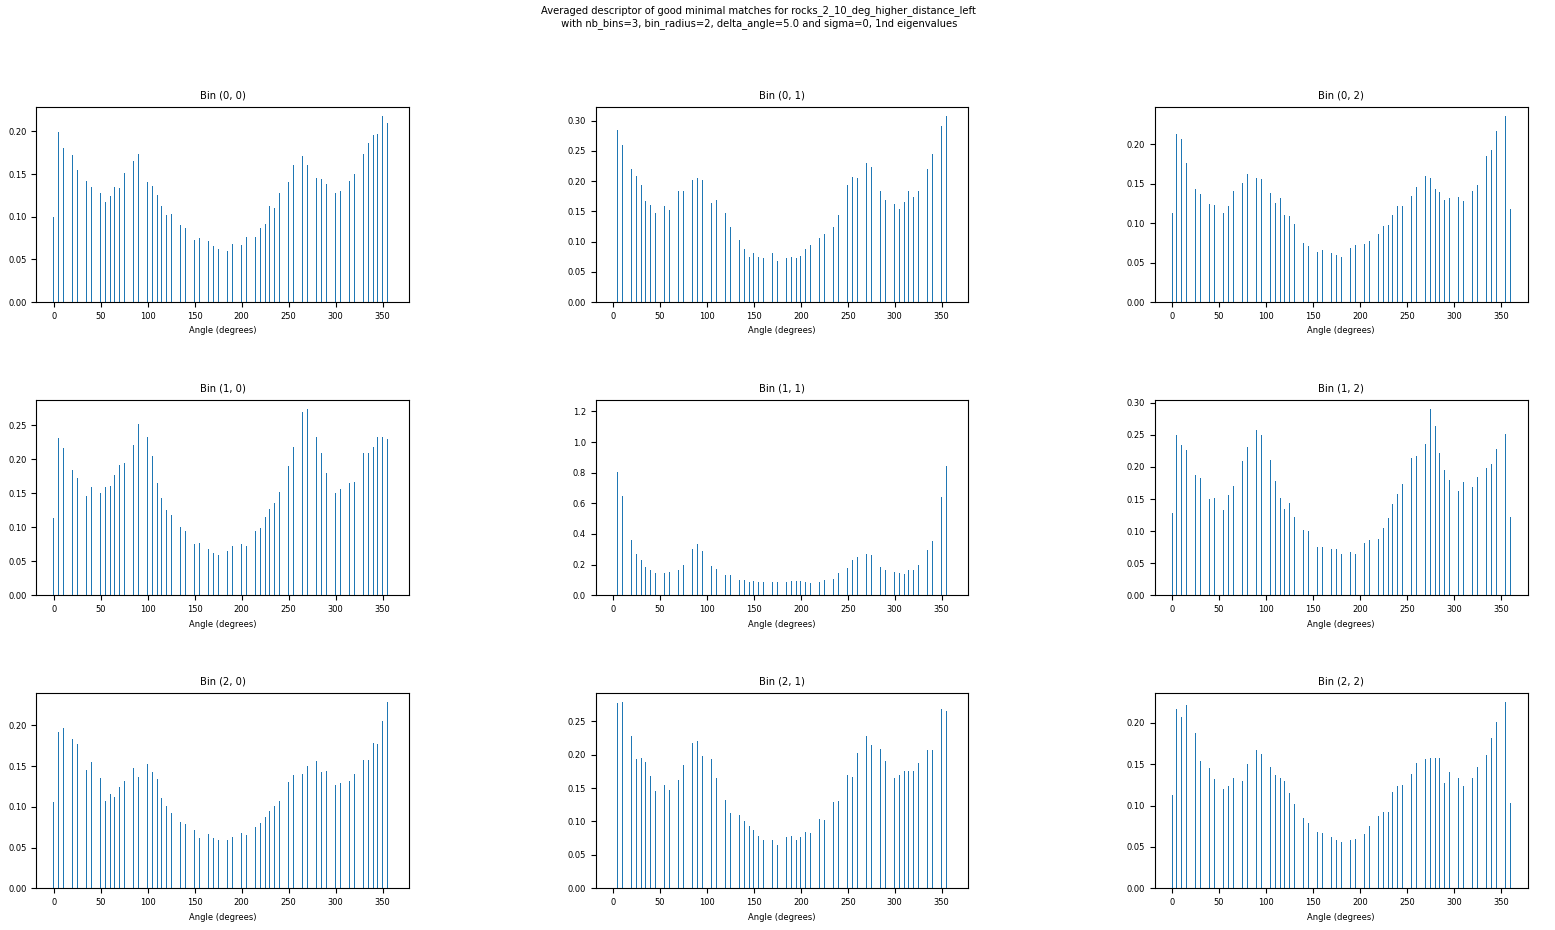
\includegraphics[width=\textwidth]{images/avg_gd_min_desc_10_left_1eig}
	\end{minipage}
	\begin{minipage}{\textwidth}
		\centering
		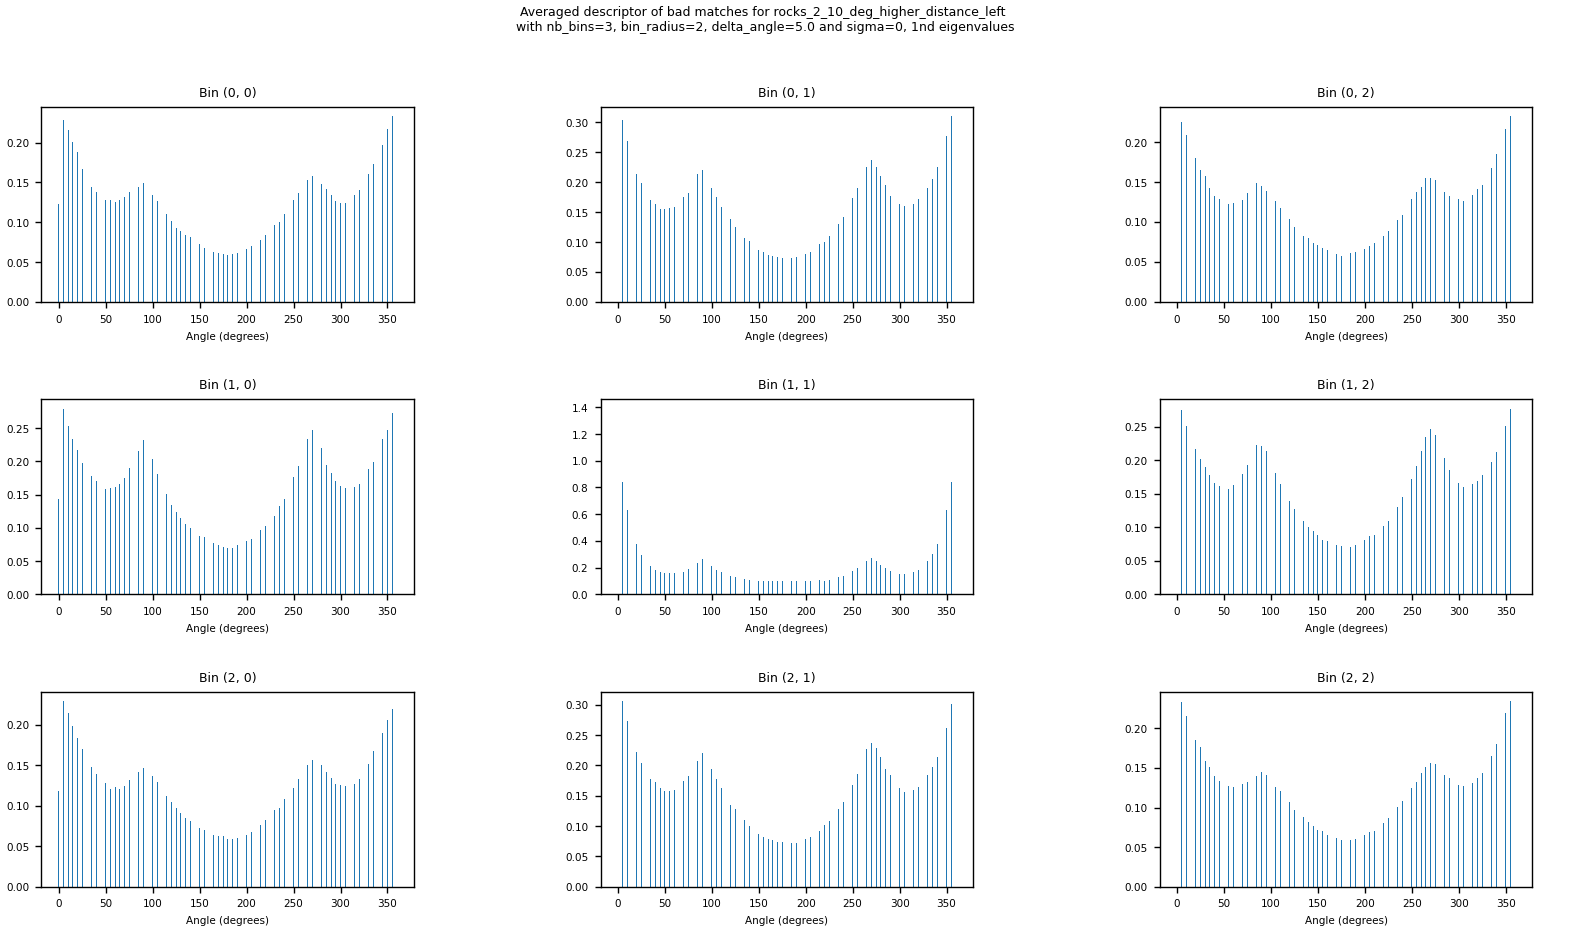
\includegraphics[width=\textwidth]{images/avg_bad_desc_10_left_1eig.png}
	\end{minipage}
	\caption{Comparaison des histogrammes spatiaux moyens de la coubure principale $1$ des bons points trouvés par \textit{HM} (à gauche, $\sim 2500$ points) et
		des mauvais points (à droite, $\sim 70000$ points) sur image Blender.}
	\label{figure:desc_comp}
\end{figure*}

\clearpage

\begin{figure*}
	\centering
	\begin{subfigure}[H]{0.45\textwidth}
		\centering
		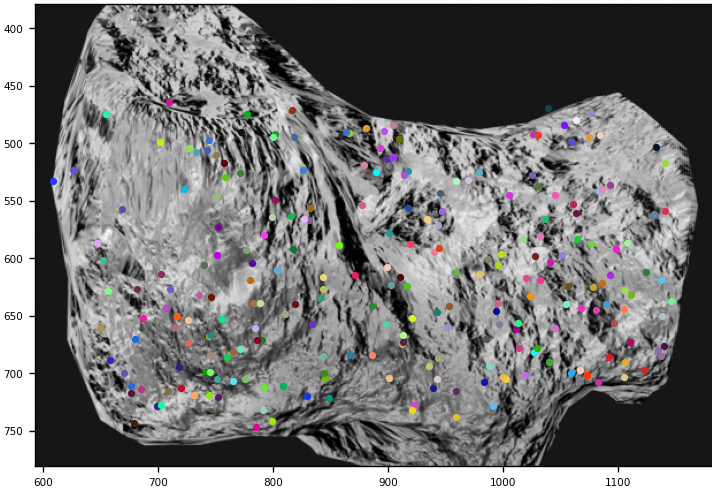
\includegraphics[width=\textwidth]{images/res1_sift_g.png}
	\end{subfigure}
	\hfill
	\begin{subfigure}[H]{0.45\textwidth}
		\centering
		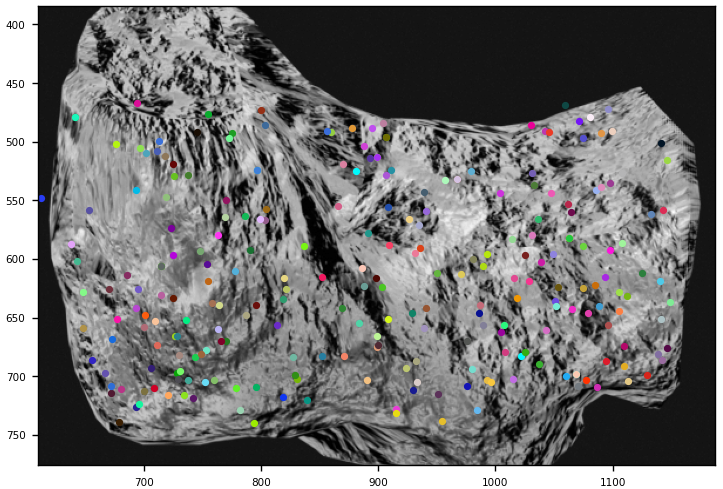
\includegraphics[width=\textwidth]{images/res1_sift_d.png}
	\end{subfigure}
	\caption{$250$ paires tirées aléatoirement parmi celles proposées par SIFT.}
	\label{figure:fig_syn_sift}
\end{figure*}

\begin{figure*}
	\centering
	\begin{subfigure}[H]{0.45\textwidth}
		\centering
		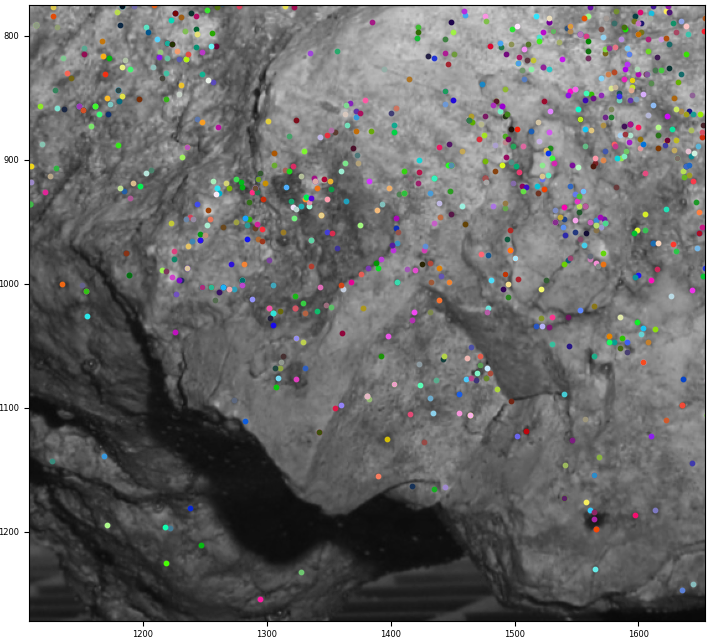
\includegraphics[width=\textwidth]{images/irl_sift_z1_g.png}
	\end{subfigure}
	\hfill
	\begin{subfigure}[H]{0.45\textwidth}
		\centering
		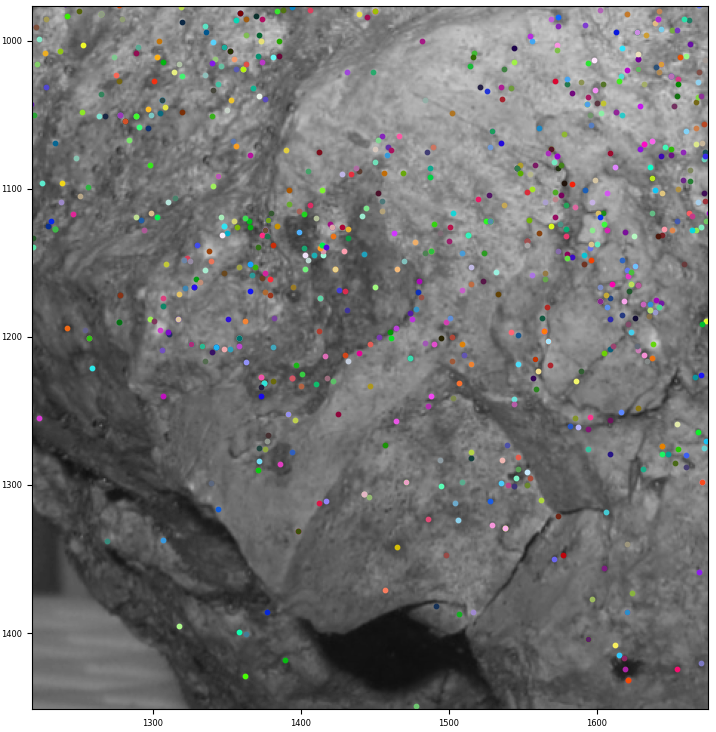
\includegraphics[width=\textwidth]{images/irl_sift_z1_d.png}
	\end{subfigure}
	\caption{Zoom sur des paires tirées aléatoirement parmi celles proposées par SIFT.}
	\label{figure:fig_irl_sift}
\end{figure*}

\clearpage

%----------------------------------------------------------------------------------------
%	 REFERENCES
%----------------------------------------------------------------------------------------

\printbibliography % Output the bibliography

%----------------------------------------------------------------------------------------

\end{document}
